% Opcje klasy 'iithesis' opisane sa w komentarzach w pliku klasy. Za ich pomoca
% ustawia sie przede wszystkim jezyk i rodzaj (lic/inz/mgr) pracy, oraz czy na
% drugiej stronie pracy ma byc skladany wzor oswiadczenia o autorskim wykonaniu.
\documentclass[declaration,shortabstract, inz]{iithesis}

\usepackage[utf8]{inputenc}

%%%%% DANE DO STRONY TYTUŁOWEJ
% Niezaleznie od jezyka pracy wybranego w opcjach klasy, tytul i streszczenie
% pracy nalezy podac zarowno w jezyku polskim, jak i angielskim.
% Pamietaj o madrym (zgodnym z logicznym rozbiorem zdania oraz estetyka) recznym
% zlamaniu wierszy w temacie pracy, zwlaszcza tego w jezyku pracy. Uzyj do tego
% polecenia \fmlinebreak.
\polishtitle    {Implementacja systemu audiowizualnego z obsługą głosową i komunikacją z komputerem pokładowym samochodu}
\englishtitle   {Implementing an audio-visual system with voice commands and communication with the engine control unit}
\polishabstract {\ldots}
\englishabstract{\ldots}
% w pracach wielu autorow nazwiska mozna oddzielic poleceniem \and
\author         {Michał Postawka}
% w przypadku kilku promotorow, lub koniecznosci podania ich afiliacji, linie
% w ponizszym poleceniu mozna zlamac poleceniem \fmlinebreak
\advisor        {dr Marek Materzok}
%\date          {}                     % Data zlozenia pracy
% Dane do oswiadczenia o autorskim wykonaniu
%\transcriptnum {}                     % Numer indeksu
%\advisorgen    {dr Jana Kowalskiego} % Nazwisko promotora w dopelniaczu
%%%%%
%%%%% WLASNE DODATKOWE PAKIETY
%
%\usepackage{graphicx,listings,amsmath,amssymb,amsthm,amsfonts,tikz}
\usepackage{graphicx}
\usepackage{placeins}
\usepackage{enumitem}
% \usepackage[utf8]{inputenc}
%
%%%%% WŁASNE DEFINICJE I POLECENIA
%
%\theoremstyle{definition} \newtheorem{definition}{Definition}[chapter]
%\theoremstyle{remark} \newtheorem{remark}[definition]{Observation}
%\theoremstyle{plain} \newthe\textbf{}orem{theorem}[definition]{Theorem}
%\theoremstyle{plain} \newtheorem{lemma}[definition]{Lemma}
%\renewcommand \qedsymbol {\ensuremath{\square}}
% ...
%%%%%

\begin{document}

%%%%% POCZĄTEK ZASADNICZEGO TEKSTU PRACY

\chapter{Wprowadzenie}

Ciężko zacząć tę pracę inaczej niż od inspiracji. Naście lat temu w kioskach można było kupić gazetki z różnymi kolekcjami podzielonymi na części. Idea była prosta - zamiast sprzedawać gotowy produkt za dużą sumę, można go było kupować po kawałku za drobne pieniądze. Popularne było składanie plastikowego szkieletu człowieka, natomiast ja wciągnąłem się w kolekcje starych amerykańskich seriali, a konkretniej  ''Nieustraszonego'' (ang. Knight Rider). Przez okres około 2 lat regularnego chodzenia do kiosku zebrałem i obejrzałem wszystkie odcinki.
No dobrze, ale co to ma do tej pracy? - można zapytać. Głównymi bohaterami są Michael Knight i jego samochód KITT. Właśnie ten pojazd stał się inspiracją całego projektu.

\begin{figure}[htp]
    \centering
    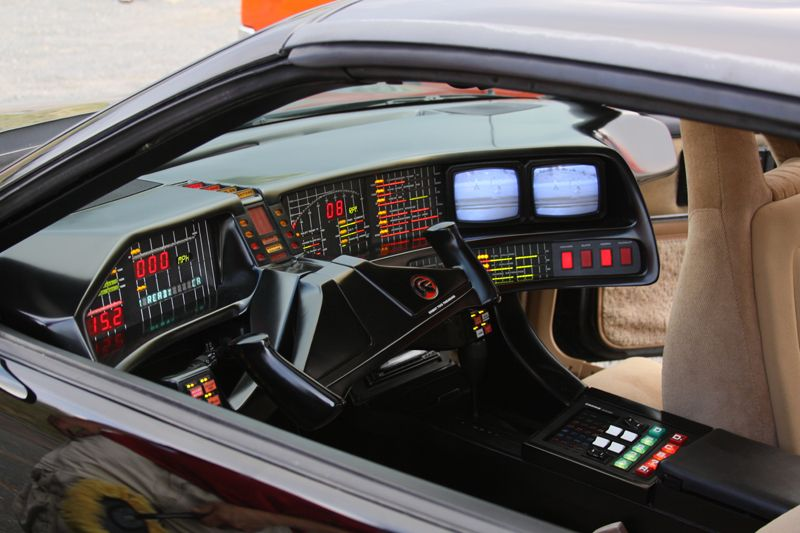
\includegraphics[width=10cm]{images/kitt_interior.jpg}
    \caption{Wnętrze KITTa}
    \label{fig:kitt}
\end{figure}

Nie byłbym w stanie dokładnie opisać KITTa, jego specyfikacja zmieniała się przez lata, ale spróbuję uchwycić to jak najlepiej. Jest to samochód wyposażony w wiele sprawnych systemów i komputer integrujący je w całość. Komputer jest więc bardzo świadomy o aktualnym stanie pojazdu i otoczenia, jest zdolny do przejęcia kontroli nad pojazdem i jego komponentami. Dzięki temu na desce rozdzielczej znalazła się masa ciekawych wskaźników i przycisków funkcyjnych. Najciekawszą częścią jest jednak moduł głosowy. Z KITTem można rozmawiać za pomocą mowy ludzkiej, prowadzić dialog, uzyskiwać potrzebne informacje i zlecać polecenia. To ta niesamowita cecha nadała mu osobowość i sprawiła, że samochód w ogóle może być postacią filmową.

Serial jest oczywiście fikcyjny, nikt nie dysponował taką technologią na początku lat 80-tych, ale wielu o tym marzyło. Nawet ja oglądając ten serial w okolicach 2010 roku nie sądziłem, żeby taki pojazd mógł istnieć na prawdę. Schowałem całą kolekcję w rogu mojego pokoju i powoli o niej zapomniałem.

10 lat później wymieniałem panel na desce rozdzielczej swojego BMW e30. Samochód powstał w dokładnie tym samym roku co serial. W rękach trzymałem moduł zegarka, prawie sześcienny z płaskim frontem. Pomyślałem, że jest podobnej wielkości i ma podobny kształt do modułu głosowego KITTa. Właściwie to było by całkiem dobre miejsce na taki moduł. Zauważyłem, że już od dłuższego czasu istnieje szereg kompetentnych asystentów głosowych. Sam korzystam z urządzenia Google Home mini, o którym mogę powiedzieć, że zapewnia dość wysoki poziom konwersacji oraz usług. Podjąłem więc decyzję -- stworzę swojego własnego asystenta, nadam swojemu samochodowi trochę osobowości i będę miał lepszą kontrolę nad stanem pojazdu.

\chapter{Specyfikacja}
\section{Samochód}
Pojazdem przeznaczonym do projektu jest BMW 316 (kod wewnętrzny BMW e30) z roku 1986.

\begin{figure}[htp]
    \centering
    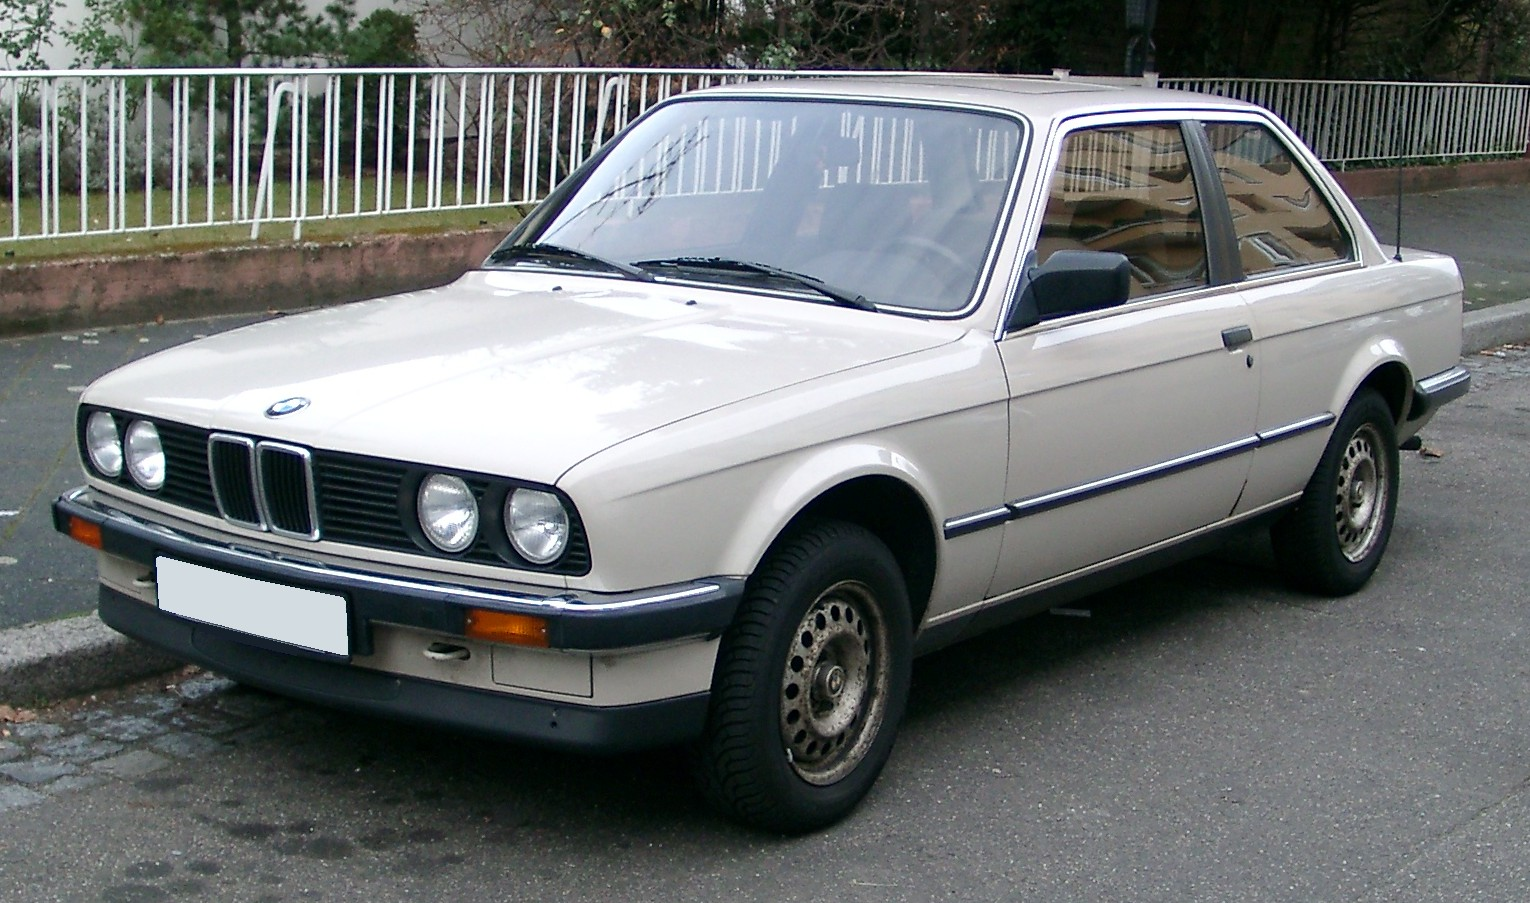
\includegraphics[width=12cm]{images/bmw_e30_front.jpg}
    \caption{BMW 316}
    \label{fig:e30_front}
\end{figure}

Na rysunku \ref{fig:e30_interior} zaznaczone są ważniejsze elementy wnętrza do których będę później wracał. Cyfrą 1 oznaczyłem przedni panel, a cyfrą 2 fabryczny zegarek.

\begin{figure}[htp]
    \centering
    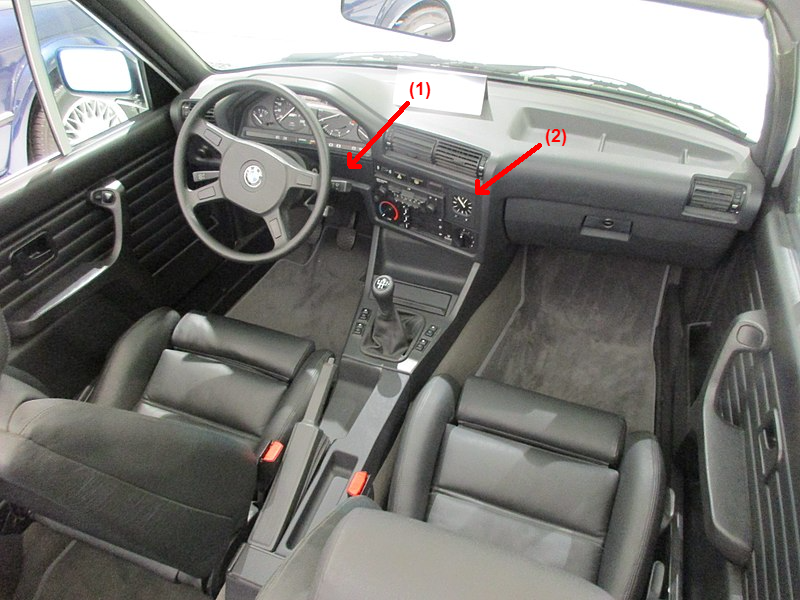
\includegraphics[width=12cm]{images/bmw_e30_interior_marked.png}
    \caption{Wnętrze BMW 316}
    \label{fig:e30_interior}
\end{figure}
\FloatBarrier

\section{Silnik}
Nie jest to pierwszy przeprowadzony przeze mnie na tym aucie projekt. Znajdująca się pod maską jednostka nie pochodzi nawet z palety dostępnych dla tego modelu silników, tylko z nowszego BMW e36 z roku 1997, wyprzedzając całą resztę o dekadę. Fabryczną jednostką sterował mechaniczny aparat zapłonowy i gaźnik. Nowy silnik (kod M44B19) sterowany jest za pomocą komputera. Pozwala to na zbieranie danych i precyzyjne kontrolowanie pracy oraz komunikację z urządzeniem zewnętrznym (w tym przypadku naszym modułem). Otwiera to zupełnie nowe możliwości.

\section{Komputer silnika}
Do sterowania został wykorzystany Bosch DME 5.2. Nie jest to otwarta platforma więc wiadomo o nim tylko to co zostało wybadane, oficjalne dane nie są udostępnione. Najbardziej interesujący będzie dla nas interfejs komunikacyjny. 

% \begin{itemize}
%     \item Samochód - BMW 316 (kod wewnętrzny BMW - e30) z roku 1986.
%     \item Silnik - 4 cylindrowa jednostka o pojemności skokowej 1.9l z nowszego modelu e36, 1997, kod M44B19.
%     \item Komputer silnika (ang. ECU) - Bosch DME 5.2
%     \item 
% \end{itemize}

% \chapter{Istniejące rozwiązania}

\chapter{Użytkowanie}
Zasilanie modułu poprowadzone zostało z obwodu akcesoryjnego samochodu. W większości pojazdów (w tym także) obwód ten zostaje zasilony w momencie przekręcenia kluczyka w stacyjce na pierwszą pozycję, i pozostaje zasilony przez wszystkie pozostałe, czasami zostaje odcięty na sam moment kręcenia rozrusznikiem, żeby zmniejszyć maksymalne obciążenie. Na tym samym obwodzie funkcjonuje fabryczne radio. Wystarczy więc wsiąść do pojazdu i przekręcić kluczyk. Po chwili oczekiwania (musi załadować się system operacyjny oraz uruchomić aplikacja) na ekranie modułu powinien pojawić się prosty analogowy zegar. Tak więc domyślną funkcją systemu jest udawanie, że jest fabrycznym zegarkiem i ukrywanie swoich dodatkowych możliwości.

System korzysta z połączenia z internetem, komputerem silnika i radiem. Jeżeli pierwsze zawiedzie, moduł ograniczy się do roli zegarka bez informowania użytkownika o problemach, zachowując dyskrecję. Jeżeli problem nastąpi na połączeniu z komputerem silnika, system powinien wciąż reagować normalnie, aczkolwiek bez podawania informacji o stanie pojazdu. Na połączenie z komputerem nie mamy wpływu, natomiast warto wiedzieć, że komputer nie otrzymuje zasilania dopóki nie przekręcimy kluczyka na pozycję drugą (zapłon). Warto więc zrobić to od razu, ale wiąże się to z większym obciążeniem i szybszym rozładowywaniem akumulatora podczas postoju, dlatego warto znać różnice. Na połączenie z internetem mamy wpływ, o ile moduł może zostać wyposażony w modem GSM/3G/LTE, wiązało by się to z utrzymywaniem kolejnego konta i kolejnymi opłatami, dlatego zdecydowałem się na inne rozwiązanie. Wbudowany w serce układy moduł WiFi stara się połączyć ze skonfigurowanym wcześniej routerem, w tym wypadku hotspotem telefonu komórkowego, który zawsze mamy przy sobie. Należy więc mieć włączony hotspot w telefonie oraz ustanowione połączenie z internetem przez sieć telefonii komórkowej. Taka obsługa urządzenia powinna zapewnić dostępność wszystkich komponentów i pełen zakres funkcji. Na koniec pozostaje nam włączyć radio i ustawić wejście na AUX. Jeżeli robiliśmy to wcześniej to powinno się to wydarzyć automatycznie po pierwszym przekręceniu kluczyka.

Po zapewnieniu powyższych warunków możemy skomunikować się z systemem (który dotychczas był dla nas tylko zegarkiem). Wpierw musimy zakomunikować, że chcielibyśmy rozpocząć konwersację. Możemy to zrobić albo za pomocą przycisku znajdującego się na desce w lewym górnym rogu panelu, albo używając słowa klucza, w tym przypadku ``Computer''. Po odebraniu takiego sygnału system zaczyna nasłuchiwać mowy. Można zadać mu w zasadzie dowolne polecenie bądź pytanie, zarówno w języku polskim jak i angielskim, chociaż domyślny będzie język angielski. Przykładowymi pytaniami mogą być:
\begin{itemize}
  \item Jaka jest dzisiaj pogoda?
  \item Opowiedz mi żart
  \item Ile lat miałby Abraham Lincoln, gdyby żył?
\end{itemize}
System nie jest wszechwiedzący ani wszechrozumny, może więc nie znać odpowiedzi bądź zwyczajnie nie rozumieć pytania. Może też źle usłyszeć i odpowiedzieć na inne pytanie, ale w większości przypadków reakcja asystenta jest na miejscu. Na czas odpowiedzi powinien zmienić się widok na ekranie komputera na przypominający moduł głosu z KITTa. Komputerowe usta powinny ruszać się wraz z wypowiadaną odpowiedzią.

Dostępne są 3 osobne widoki, domyślny zegar, usta asystenta oraz ``dashboard'' czyli monitorowanie aktualnego stanu silnika. Żeby przełączyć się miedzy nimi należy wydać polecenie takie jak:
\begin{itemize}
  \item switch to dashboard
  \item show clock
  \item change view to voice view
\end{itemize}
Naturalne kombinacje powyższych komend też powinny zadziałać.

\chapter{Konstrukcja}
\section{Część fizyczna}
W tej części znajduje się omówienie projektu od strony sprzętu (ang. hardware) i montażu.
\subsection{Komponenty}
\begin{description}[style=nextline]
  \item[Raspberry Pi - model 4B w wersji 2Gb pamięci RAM]
    Jest to jednopłytkowy komputer z procesorem typu ARM z niskim poborem prądu.
    Można by wybrać wiele innych komputerów do tego projektu, ten zapewnia wystarczającą wydajność i rozszerzalność, jest wprost kompatybilny z ekranem i ma najsolidniejsze wsparcie ze wszystkich dostępnych na rynku produktów.
  \item[Karta microSD - SanDisk Extreme 32gb zgodny z UHS-1]
    Warto wybrać jak najlepszą kartę pamięci (ona pełni rolę pamięci stałej naszego urządzenia), ponieważ od jej szybkości zależy chociażby czas uruchomienia całego urządzenia (i różnice między wolnymi a szybkimi kartami bywają tutaj bardzo duże, nawet 10-krotne). Ważne jest też, żeby karta miała odpowiednią wytrzymałość, gdyż karty SD nie są przeznaczone do takiego użytku (ich prawidłowe miejsce jest w aparatach fotograficznych) i potrafią utracić dane pod wpływem wielokrotnych zapisów systemu operacyjnego, bądź nagłych utrat zasilania.
  \item[Kamera / mikrofon - Sony PlayStation Eye]
    To chyba mój ulubiony element, sprzedawana jako dodatek do Sony PlayStation 3 kamera z 4-rema mikrofonami. Z racji, że producenci konsol do gier nie zarabiają największych pieniędzy (często nawet tracą) na samych konsolach, ale na koncesji z każdej sprzedanej gry, ceny konsol i sprzętu towarzyszącego są jak najniższe, a jakość bardzo wysoka. Dobrze wpływa na cenę też masowość produkcji. Urządzenie to można więc kupić bardzo tanio, jest bardzo popularne i da się je bez problemu podłączyć do Raspberry Pi (istnieją dostępne sterowniki). Mikrofon jest zdecydowanie najlepszy w swojej klasie, porównywałem go z kilkoma innymi, w tym dedykowanymi do Raspberry Pi (od ReSpeaker) i dużo lepiej sobie radził z rozpoznawaniem mowy, w szczególności w zaszumionych środowiskach (takich jak wnętrze jadącego samochodu).
  \item[Ekran IPS 3.5'' - Waveshare 12824]
    Moją początkową ideą było stworzenie wyświetlacza przypominającego moduł głosu KITTa z diod LED (prototyp opisałem poniżej), ale zrezygnowałem z niego z powodu ograniczonych funkcji oraz trudności ładnego wykończenia, tak żeby całość dobrze komponowała się z wnętrzem auta i nie wyglądała amatorsko. Nie zamierzałem natomiast rezygnować z funkcji modułu głosu (w znaczeniu wizualnym), chciałem więc żeby ekran nie stwarzał wrażenia wyblakłego taniego TFT z początków istnienia LCD, tylko żeby potrafił wyglądać jak indywidualne LEDy. Musiał to być ekran wysokiej jakości wykonany w dobrej technologii. Idealnym wyborem byłby ekran OLED, ale nie znalazłem żadnego który nie byłby ani za mały względem wielkości otworu, ani za duży (całość nie może być znacząco większa niż oryginalny zegarek). Drugą najlepszą technologią płaskich ekranów jest LCD IPS, zapewniając żywe kolory i szerokie kąty widzenia, ekran 3.5 cala od Waveshare okazał się mieścić idealnie i pasował wprost na Raspberry Pi, tworząc zwartą całość.
  \item[Ładowarka samochodowa USB 3A]
    W porównaniu do poprzednich modeli Raspberry Pi 4 charakteryzuje się dość wysokim poborem prądu, większym niż można oczekiwać od standardowej ładowarki USB, a trzeba zasilić także ekran. Najtańsza ładowarka z funkcją QuickCharge 3 okazała się trafiona i spełniła oczekiwania mocy.
  \item[Interfejs diagnostyczny OBD2 kompatybilny z BMW OBD1]
    Interfejs dostępny w samochodzie (OBD1) jest częściowo kompatybilny z ustandaryzowanym później OBD2. Jest też dużo mniej popularny, występuje tylko w samochodach dostępnych przez pojedyncze lata produkowanych przez BMW, natomiast OBD2 jest używane w samochodach wszystkich marek od lat 2000 do dziś. Da się natomiast kupić interfejs wspierający BMW OBD1, potrzebna jest tylko przejściówka. Taki zestaw daje możliwość komunikacji, ale program diagnostyczny również musi wspierać BMW OBD1, co nie jest popularne.
  \item[Stelaż montażowy modułu w miejsce zegarka]
    Takiego elementu nie ma niestety dostępnego w sprzedaży. Fabryczny stelaż mocujący moduł zegarka do panelu deski rozdzielczej nie nadawałby się do naszego modułu o innych wymiarach. Mocowanie byłem zmuszony zaprojektować i stworzyć samemu. O projektowaniu więcej w sekcji~\ref{section:3d}.
\end{description}








% \begin{figure}[htp]
%     \centering
%     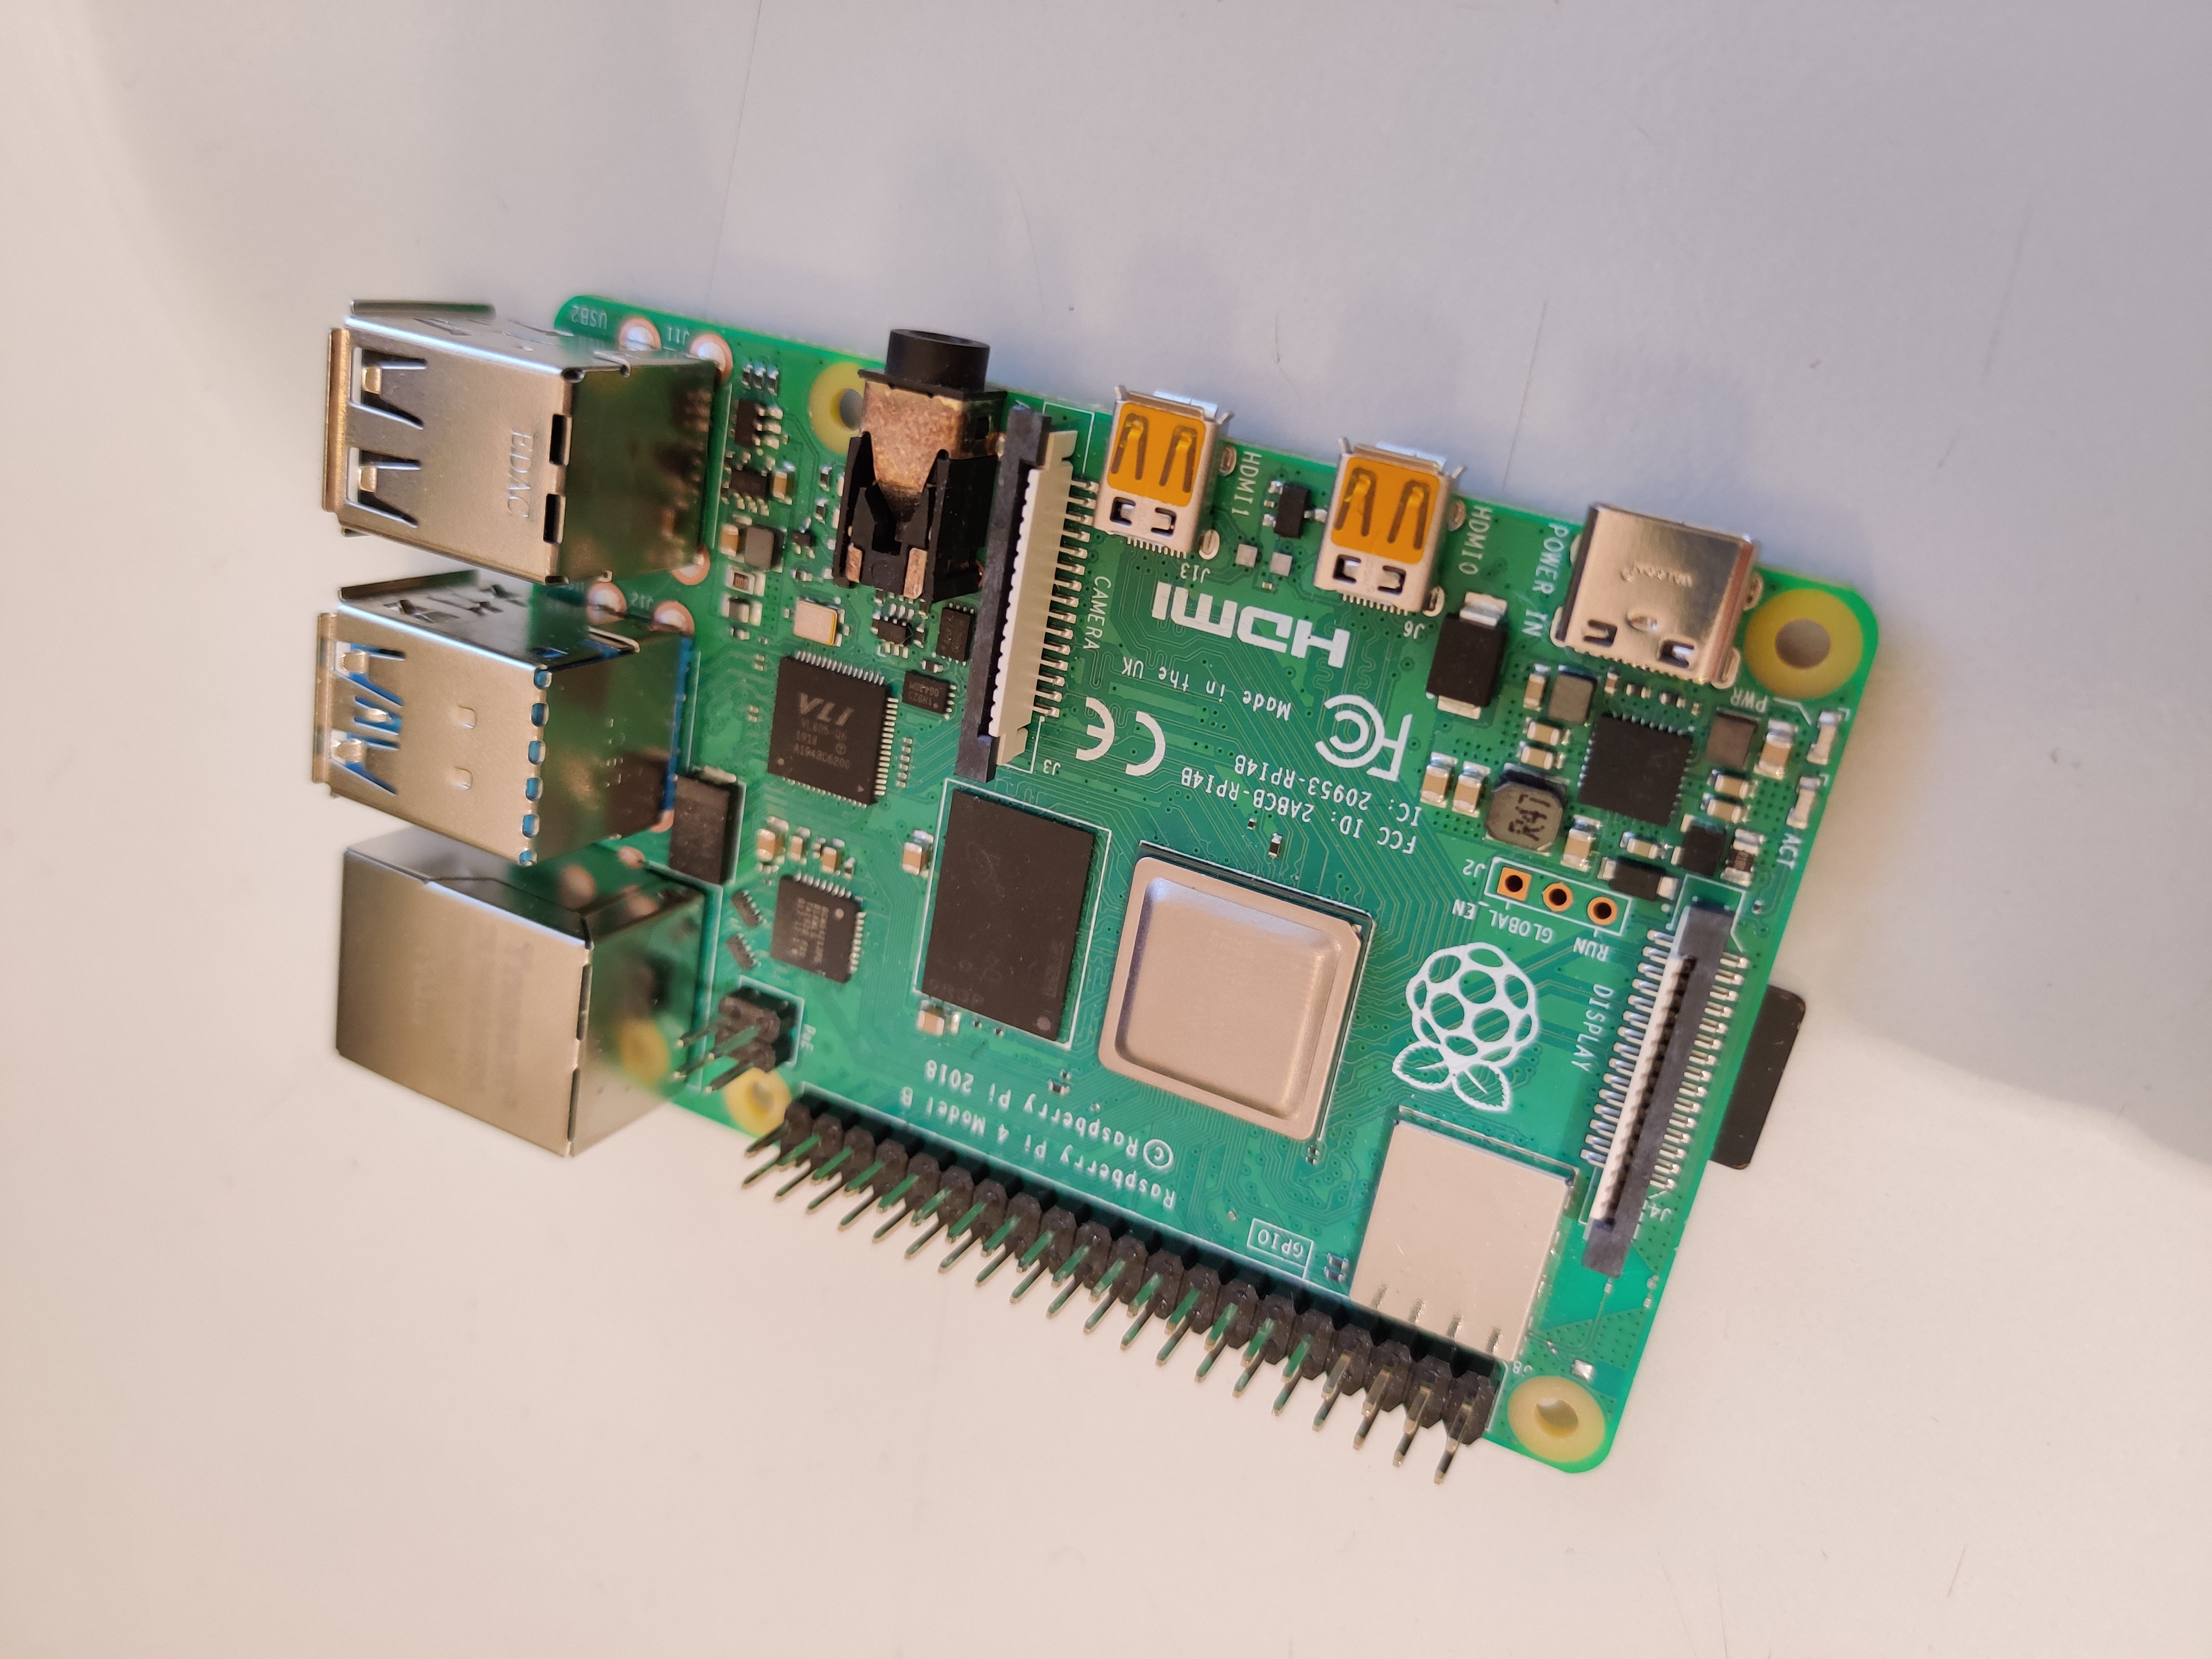
\includegraphics[
%         width=12cm,
%         keepaspectratio
%     ]{images/raspberry_vertical.jpg}
%     % \caption{}
%     \label{fig:rpi}
% \end{figure}
% \begin{figure}[htp]
%     \centering
%     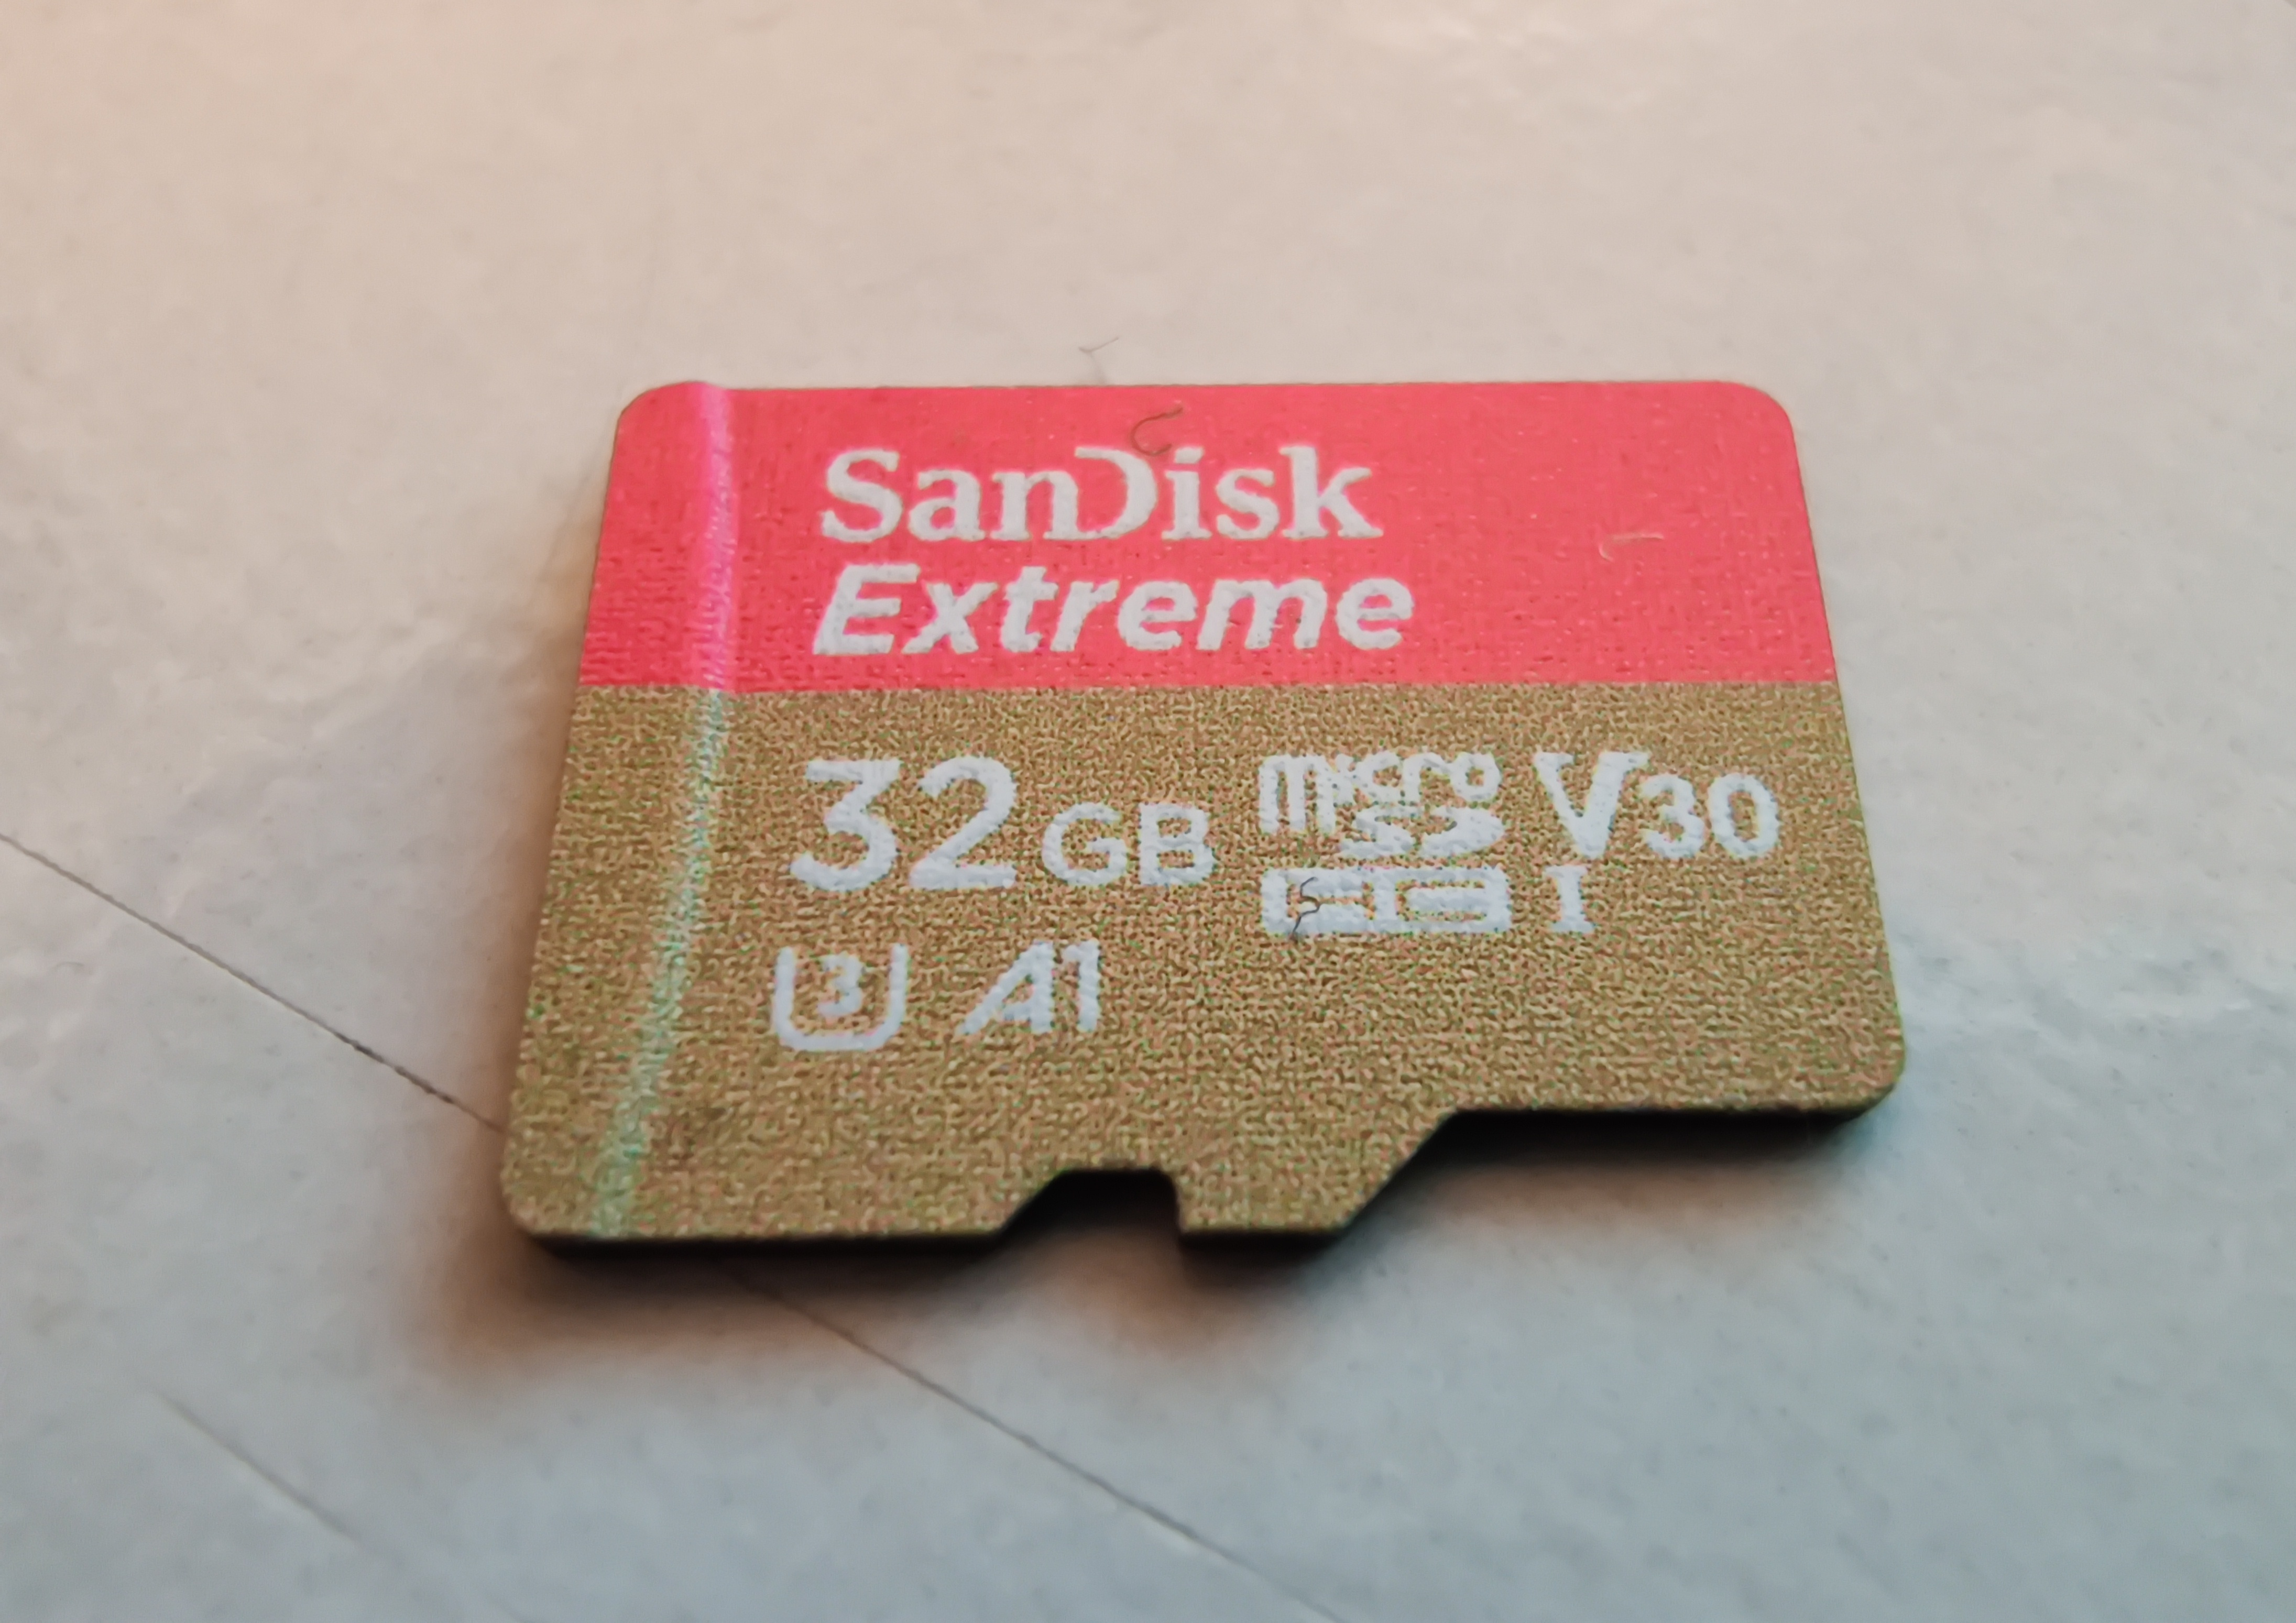
\includegraphics[
%         width=12cm,
%         keepaspectratio
%     ]{images/sandisk_microsd.jpg}
%     \label{fig:microsd}
% \end{figure}
% \begin{figure}[htp]
%     \centering
%     \includegraphics[
%         width=12cm,
%         keepaspectratio
%     ]{images/pseye.png}
%     \label{fig:pseye}
% \end{figure}
% \begin{figure}[htp]
%     \centering
%     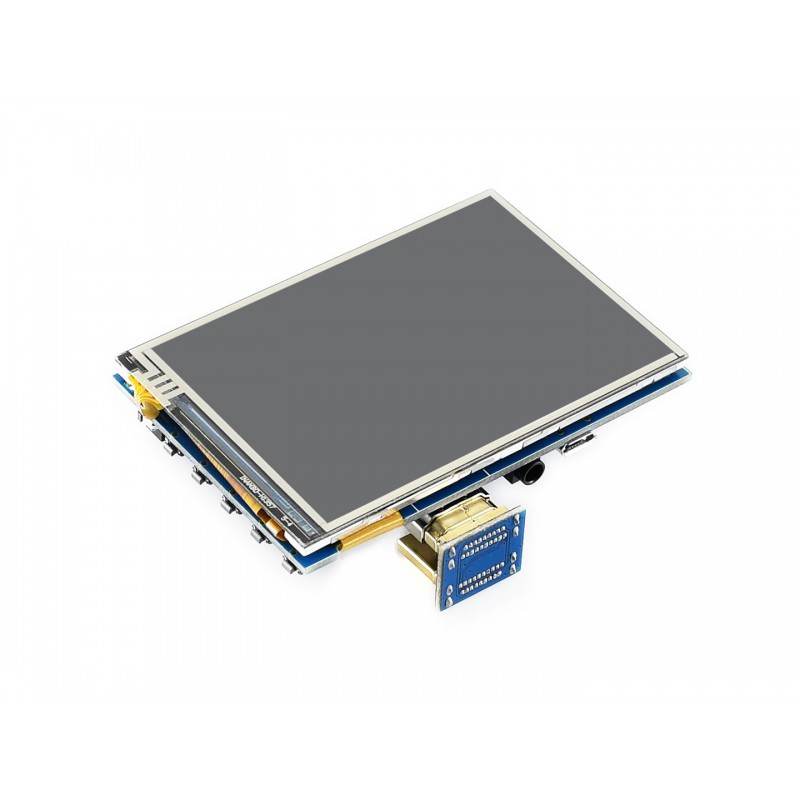
\includegraphics[
%         width=12cm,
%         keepaspectratio
%     ]{images/waveshare_lcd_35.jpg}
%     \label{fig:screen}
% \end{figure}
% \begin{figure}[htp]
%     \centering
%     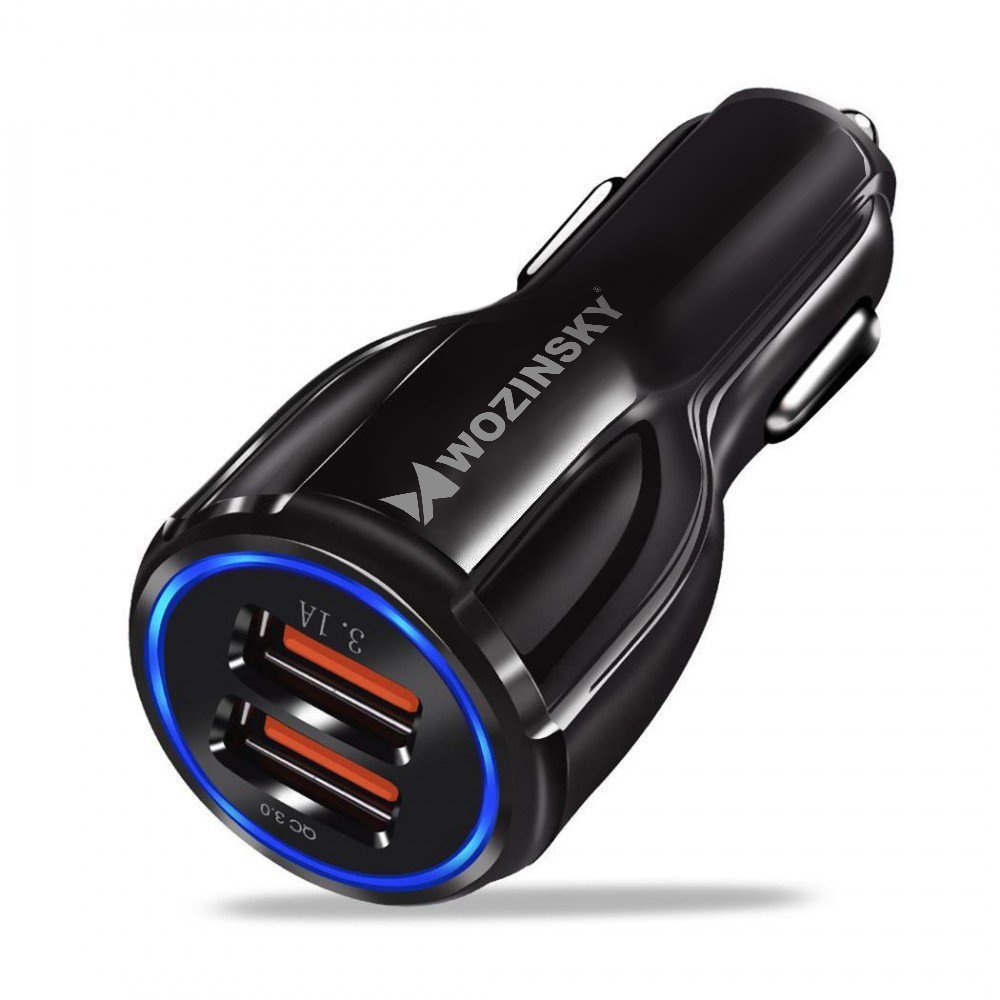
\includegraphics[
%         width=12cm,
%         keepaspectratio
%     ]{images/charger.jpg}
%     \label{fig:charger}
% \end{figure}
% \begin{figure}[htp]
%     \centering
%     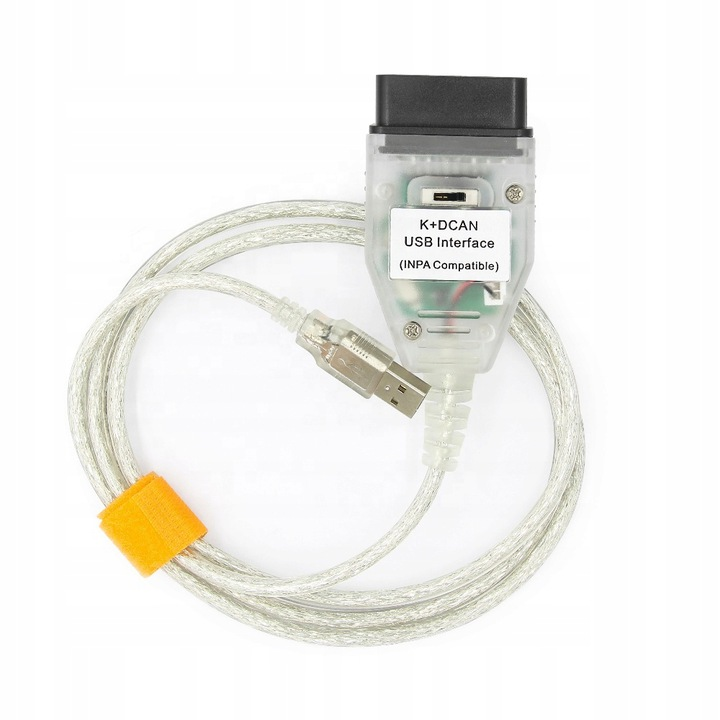
\includegraphics[
%         width=12cm,
%         keepaspectratio
%     ]{images/obd2_inpa.jpeg}
%     \label{fig:obd}
% \end{figure}
  
  
\subsection{Drukowanie 3D}
    Do wydrukowania modeli użyłem drukarki bazowanej na Prusa i3 na stalowej ramie. Jest to jedna bardziej podstawowych drukarek 3D dostępnych na rynku, drukuje w technologi FDM / FFF, czyli nakładanie rozgrzanego pół-płynnego filamentu warstwa po warstwie. Osiągnięcie sensownych wydruków wymagało długiej zabawy z parametrami drukarki, takimi jak prędkości posuwów, wysuwu fillamentu czy temperatury głowicy bądź podstawy. Zdecydowałem się na wykorzystanie plastiku ABS, który jest delikatnie mocniejszy i lepiej znosi ciężkie warunki takie jak wysoka temperatura wewnątrz pojazdu bądź promienie UV, aczkolwiek wymaga przy drukowaniu wyższych temperatur i trudniej jest uzyskać ładny wydruk niż w technologii materiałowej PLA (która jest raczej typowa dla takich drukarek). Po wielu próbach osiągnąłem maksimum lokalne jakości wydruku, ale muszę przyznać że było to raczej minimum akceptowalności, zmuszony zostałem do pogrubienia wielu elementów gdyż moje wczesne projekty łamały się i rozwarstwiały.


\subsection{Wdrażanie}
    Przyszedł czas złożyć wszystko w całość. Ekran wprost spina się z Raspberry w jeden obiekt. Następnie przykręcenie stelażu do panelu od tyłu. Wtedy pojawiły się pierwszy problem. Śruby mocujące stelaż mają dość wysoki łeb (około 3mm). Jedna z nich miała swoje miejsce tuż przed portem zasilania USB typ C. Nie był to nawet głupi błąd przy projektowaniu, nie dało się uniknąć tej kolizji przez inne umiejscowienie przestrzenne modułu, nie było na to miejsca. Po długich walkach i eksperymentowaniu z wieloma kablami i wtyczkami nie znalazłem dobrego rozwiązania. Zostałem zmuszony do wykręcenia tej śruby, tak że moduł trzyma się teraz na trzech i tylko opiera w czwartym miejscu\footnote{Z resztą komu się nigdy nie zdarzyło rozebrać coś i złożyć tak, że na stole wciąż pozostały niewkręcone nigdzie śrubki.}. Okazało się to być równie stabilne i wystarczająco mocne. Oryginalny panel z zegarka (maskownica) musiałem spłaszczyć przy pomocy szlifierki, tak aby ładnie przylegał do ekranu (wystawały z niego zaczepy, na które teraz nie było miejsca) i podkleiłem taśmą dwustronną. Następnie nakleiłem panel na ekran tak, żeby wyglądał jak fabryczny moduł.
    
    Teraz należało znaleźć miejsce na mikrofon. Dla najlepszego efektu powinien znajdować się jak najbliżej ust kierowcy. Największą trudnością było znalezienie miejsca które mógłbym wykorzystać bez dużej ingerencji w budowę deski rozdzielczej. Wybrałem miejsce opisane cyfrą (1) na rysunku \ref{fig:e30_interior}. Najpierw rozebrałem kamerę do poziomu płytki z której wystawały 4 mikrofony. Z funkcji rejestracji obrazu nie zamierzałem korzystać, więc wszystko poza mikrofonami zakleiłem taśmą izolacyjną. Na mikrofony nałożyłem maskownicę która była elementem pośrednim między obudową PsEye a elementami mikrofonów. Następnie wywierciłem w panelu (tym oznaczonym cyfrą 1) 4 otwory o odstępach i wielkościach odpowiadających tej maskownicy. Należało jeszcze wykroić nożem trochę pianki z deski pod panelem, żeby zrobić miejsce dla płytki. Na szczęście wszystko się ładnie zmieściło i wygląda prawie fabrycznie po zmontowaniu. Poprowadzenie kabla pod deską do modułu nie było już problematyczne.
    
    Pozostało połączyć moduł z radiem za pomocą kabla jack oraz z interfejsem diagnostycznym, a interfejs z wiązką silnika, co przebiegło bezproblemowo. Natomiast na sam koniec przy wkładaniu całego przedniego panelu okazało się, że karta pamięci włożona do slotu Raspberry Pi wystaje trochę poza obrys. Początkowo zignorowałem sprawę i próbowałem wmanewrować panel na swoje miejsce, uszkadzając przy tym kartę pamięci! Zmuszony więc byłem wszystko zainstalować od nowa, a na kartę zrobić w desce miejsce nożykiem (jest to niewidoczne z zewnątrz).
\section{Tworzenie modeli 3D}
\label{section:3d}
\section{Środowisko testowe} % może do części fizycznej?
\section{Część programistyczna}

%%%%% BIBLIOGRAFIA

%\begin{thebibliography}{1}
%\bibitem{example} \ldots https://pl.pinterest.com/pin/283656476514503341/
%\end{thebibliography}

\end{document}
